\lab{Parallel Computing with $\texttt{ipyparallel}$}{Parallel Computing with $\texttt{ipyparallel}$}
\objective{(TODO: Awesome objective coming!)}
\label{lab:parallel1}

\section*{Why Parallel Computing?}
When a single processor takes too long to perform a computationally intensive task, there are two simple solutions.
The first is simply to build a faster processor.
Unfortunately, physics gets in the way.
In particular, the problem of heat dissipation has kept processor speeds from increasing as quickly in recent years as they did in the past.
The second solution is to have mutiple processors work together on the same task.
This is the main idea behind parallel computing. Essentially, a `supercomputer' is made up of many normal computers, each with its own memory.

Today, high computing performance is achieved using many processors.
These processors communicate with each other and coordinate their tasks with a message passing system. The details of this message passing system, MPI, will be the topic of the next lab.

In this lab, we will become familiar with some of the basic ideas behind parallel computing.

\section*{Serial Execution vs. Parallel Execution}
Up to this point, all the programs you have written run in \emph{serial}. This means that each command is executed one line at a time. The following exercise will help you visualize what is happening.

\begin{problem}
If you are working on a Linux computer, open a terminal and execute the \li{htop} command. (If \li{htop} is not on your system, install it using your default package manager). When opening this program, your terminal should see an interface similar to Figure \ref{fig:htop}. The numbered bars at the top represent each of the cores of your processor and the workload on each of these cores.

Now, run the following python code with your terminal running \li{htop} still visible. The sole purpose of the following code is to create a computationally intensive function that runs for about 15 seconds.

\begin{lstlisting}
import numpy as np
for i xrange(10000):
    np.random.random(100000)
\end{lstlisting}

You should have seen one of the cores get maxed out at 100\%. It is also possible that you saw the load-carrying core switch midway through the execution of the file. This is evidence one indicator that our script is being executed in serial -- one line at a time, one core at a time.
\end{problem}

\begin{figure}
    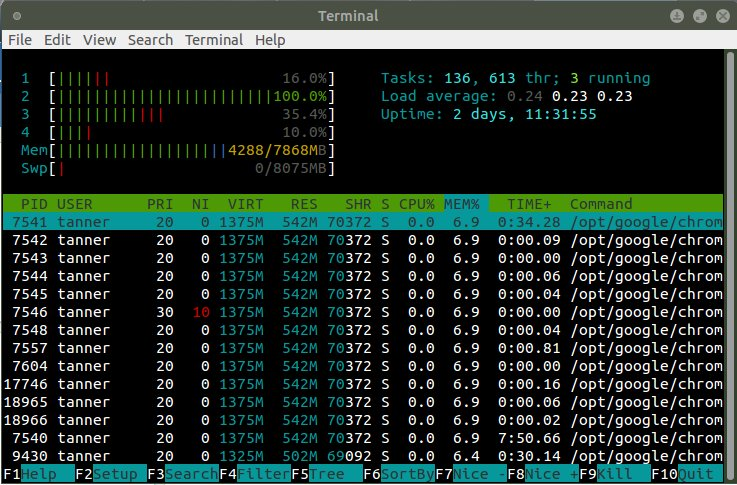
\includegraphics[width=\textwidth]{active.jpg}
\caption{An example of \li{htop} with a computationally intense python script running.}
\label{fig:htop}
\end{figure}

As you saw in the exercise above, only one of the cores was carrying the load at a time. This means that we are only using a fraction of the computer's resources. When working on a personal computer, this would often be to your benefit. Dividing jobs among multiple cores is part of what makes smooth multitasking possible. However, in the event you wish to devote all the computer's resources to executing your code, we employ the help of the \li{ipyparallel} module. In theory, you can make your code run $N$ times faster when executing in parallel where $N$ is the number of cores

\section*{The $\texttt{ipyparallel}$ Module}
We will begin our discussion on parallel computing by learning about the \li{ipyparallel} module. Even though this may not be the fastest parallel computing framework available, it is very easy to take advantage of all the cores on your computer with relatively little code. As mentioned before, you cannot expect your code to magically run faster if you requests the usage of more cores on your computer. You have to specify what happens on each core. This concept is key to understanding parallel computing.

\subsection*{Installation and Initialization of $\texttt{ipyparallel}$}

If you have not already installed \li{ipyparallel}, you may do so using the conda package manager.

\begin{lstlisting}
$ conda update conda
$ conda update anaconda
$ conda install ipyparallel
\end{lstlisting}

With \li{ipyparallel} installed, we can now initialize an IPython cluster. We won't go too much into the architecture of the IPython cluster, but if you are interested in learning more, visit \url{https://ipyparallel.readthedocs.io/en/latest/intro.html#architecture-overview}.

Now to initialize an IPython cluster, run the following code:

\begin{lstlisting}
$ ipcluster start
\end{lstlisting}

This will start a cluster with one engine per processor. If you would like to specify the number of engines to initialize, run the following:

\begin{lstlisting}
# start a cluster with 8 engines.
$ ipcluster start --n 8
\end{lstlisting}

If you choose to explicitly specify the number of engines, it is not optimal to initialize more engines than you have processors. Doing so would require multitasking on each processor instead of having each processor dedicated to one task.

If you are more accustomed to using Jupyter Notebooks, you may have noticed the ``Clusters" tab. You can start an IPython cluster in this tab after enabling the \li{ipcluster} notebook extension.

\begin{lstlisting}
$ ipcluster nbextension enable
\end{lstlisting}

\begin{problem}
Initialize an IPython cluster with an engine for each processor. As you did in the previous problem, open \li{htop}. Run the following code and examine what happens in htop.

\begin{lstlisting}
from ipyparallel import Client
client = Client()
dview = client[:]

dview.execute("""
import numpy as np
for i in xrange(10000):
    np.random.random(100000)
""")
\end{lstlisting}

The output of \li{htop} should appear similar to Figure \ref{fig:htop_cluster}. Notice that all of the processors are being utilized to run the script.
\end{problem}

\begin{figure}
    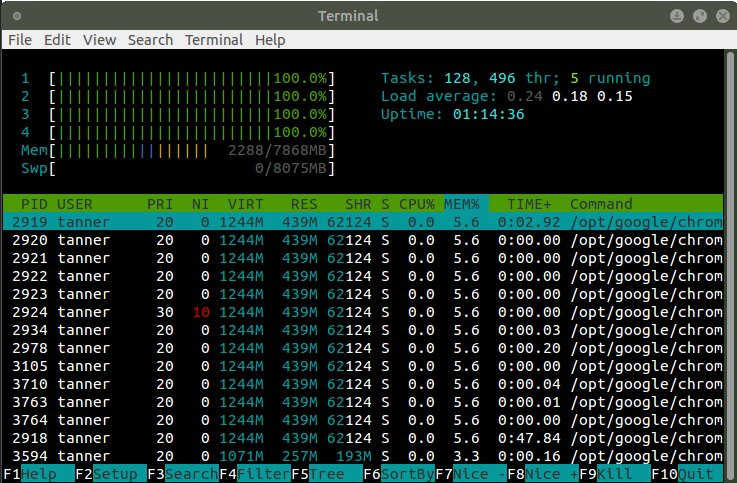
\includegraphics[width=\textwidth]{cluster_active.jpg}
\caption{An example of \li{htop} with a computationally intense python script running in parallel.}
\label{fig:htop_cluster}
\end{figure}

We have now ensured that our IPython cluster is successfully executing on all engines. Now we will dive into the details of how we can utilize the cluster and discuss the syntax to use.

\section*{Syntax for $\texttt{ipyparallel}$}
The basic framework for \li{ipyparallel} revolves around a \li{DirectView} or a \li{LoadBalancedView}.
A \li{DirectView} is the object through which we communicate with each of the engines. You have control over which variables are pushed to each engine and what functions are performed. A \li{LoadBalancedView} takes the commands that are being executed and does its best to distribute the load evenly across all the engines.

For the purposes of having more control over each engine, we will focus on the \li{DirectView} in this lab. To initialize a \li{DirectView}, run the following code:

\begin{lstlisting}
>>> from ipyparallel import Client
>>> client = Client()

# verify the dview has been generated correctly.
#   On my system, I have 4 processors.
>>> client.ids
[0, 1, 2, 3]

# initialize DirectView
>>> dview = client[:]
\end{lstlisting}

\subsection*{Variables on Different Engines}
When using multiple processors, each engine has its own namespace. Therefore, just because a variable has been initialized does not mean that each engine is aware of that variable. You must initialize these variables explicitly on each engine. There are a few different ways to do this.

\begin{lstlisting}
# To share the variable `a' across all engines
>>> a = 10
>>> b = 5
>>> dview["a"] = a
>>> dview["b"] = b

# Or alternatively,
>>> dview.push({'a':a, 'b':b})

# To ensure the variables are on engine 0
>>> client[0]['a']
10

>>> client[0]['b']
5
\end{lstlisting}

The code you just ran is the easiest way to get individiual values on each of the engines. We will discuss some other methods a bit later in this lab. We will now move on to doing some simple computations in parallel.

\subsection*{The $\texttt{apply()}$ and $\texttt{apply\_sync()}$ Methods}
To execute functions on each of the engines, we can use the \li{apply()} or the \li{apply\_sync()} methods.  The difference between \li{apply()} and \li{apply\_sync()} comes down to blocking. If a function is executed with blocking, you will be unable to run any other commands until the function has finished. If a function is run without blocking, you can execute other commands while that function is still computing its result. The \li{apply()} methods executes without blocking and the \li{apply\_sync()} method executes with blocking. The following code box describes how this is done:

\begin{lstlisting}
>>> def add():
...     return a+b

# Runs add() without blocking (in background)
>>> result = dview.apply(add)

# Checks to see if the output is ready
>>> result.ready()
True

# Retrieves output
>>> result.get()
[15, 15, 15, 15]

# Runs add() with blocking
>>> dview.apply_sync(add)
[15, 15, 15, 15]
\end{lstlisting}

You can also pass variables into your function as part of call to \li{apply\_sync()}. Consider the following example:

\begin{lstlisting}
>>> def add(x, y):
...    return x+y

>>> dview.apply_sync(add, 3, 6)
[9, 9, 9, 9]
\end{lstlisting}

\begin{problem}
To this point, the examples of what you can do with parallel computing may not have been very convincing since we were just getting the same answer on each engine. In this problem, we will make better use of each of the engines.

Using \li{apply\_sync()}, draw 1,000,000 samples from a standard normal distribution. Report the mean, max, and min for draws on each individual engine. For example if you have four engines running, your output should look like:
\begin{lstlisting}
means = [0.0031776784, -0.0058112042, 0.0012574772, -0.0059655951]
maxs = [4.0388107, 4.3664958, 4.2060184, 4.3391623]
mins = [-4.1508589, -4.3848019, -4.1313324, -4.2826519]
\end{lstlisting}

In theory, using parallel computing for this problem should be approximately $n$ times faster where $n$ is the number of engines you are using.
\end{problem}

\begin{problem}
Now let's do a problem that is a bit more computationally intensive. Define the random variable $X$ to be the maximum out of a $N$ draws from the standard normal distribution. Take 500,000 draws from this distribution and plot the draws in a histogram. The resulting histogram will approximate the p.d.f. of $X$.

Write your function in such a way that each engine will carry an equal load. Also write your function in such a way that it is flexible to the number of engines that are running. HINT: Remember that you can get a list of all available engines using \li{clients.ids}.
\end{problem}

\subsection*{The $\texttt{scatter()}$ and $\texttt{gather()}$ Methods}
There are many situations where we would want to spread a dataset across all the available engines. This way, we can have a function work on each of these portions of the dataset. In its simplest form, this is the basis of MapReduce. We will address MapReduce in more detail in a future lab.

We will first introduce an example of \li{scatter()} and explain the proper usage in more detail throughout the example.

\begin{lstlisting}
# Initialize the dataset to scatter
>>> a = np.arange(10)

# Scatter the data. The pieces of the data will be
#   named "a_partition" on each of the engines.
>>> dview.scatter("a_partition", a)

# Verify that the data has been successfully scattered
#    Notice that the data has been scattered as
#    equally as possible.
>>> client[0]["a_partition"]
array([0, 1, 2])

>>> client[1]["a_partition"]
array([3, 4, 5])

>>> client[2]["a_partition"]
array([6, 7])

>>> client[3]["a_partition"]
array([8, 9])
\end{lstlisting}

Now that the \li{a_partition} variable has been initialized on each engine, we can now execute functions that depend on this variable. Consider the following simple example using the \li{execute()} method.

\begin{lstlisting}
# Pass a string with the Python code that we wish to run
#   on each engine. This code will simply sum the entries
#   in "a_partition"
>>> dview.execute("""
... b = a_partition.sum()
... """)
\end{lstlisting}

\begin{info}
If you are using a Jupyter Notebook, there is a built in magic function that is analagous to \li{dview.execute()}. If you put the \li{\%\%px} magic at the beginning of a cell of code, that cell of code will be executed on each engine. This tool is very useful for designing and debugging parallel algorithms.
\end{info}


We have now computed the sum of each of these pieces of the data and stored the result in the variable $b$. Now how can we gain access to all these results? We use the \li{gather()} method.

\begin{lstlisting}
# gather all the 'b' values into a list.
>>> b_list = dview.gather("b", block=True)
[3, 12, 13, 17]

>>> sum(b_list)
45
\end{lstlisting}

To summarize, this example has taken a piece of data, scattered it to all available engines, performed a computation on each of these pieces of data, then gathered the results back to the controller.

\begin{problem}
All of the examples that we have done in this lab up to this point may have seemed quite simplistic. However, we will now apply all these examples to a real-world example.

Many natural language processing (NLP) problems naturally extend to a parallel computing architecture. In many situations, we will have a function we want to apply to a piece of text, whether that be a sentence, paragraph, or an entire document. An efficient way to handle these problems is to scatter the data to all available engines, perform the calculations, then gather the results.

The introductory step to latent symantic analysis is to create a occurance matrix based on the bag-of-words model. At a high level, the bag-of-words model gives us insight as to the topic of a given document. It can also be used to measure the similarity between two documents.

The occurrence matrix has the ids for the different documents as the rows and the different words in the vocabulary as the columns. Then the $ij$-th entries of this matrix is the number of times the $j$-th word appears in the $i$-th document. For example, consider the following example:

Say we have the following 4 pieces of text:
\begin{enumerate}
    \item the rose is red
    \item the violet is blue
    \item my car is red
    \item i have a red rose and a red car
\end{enumerate}

It is common to remove \emph{stopwords} or the most common words in the language. We can get a list of stopwords by running:
\begin{lstlisting}
>>> from nltk.corpus import stopwords
>>> set_stopwords = set(stopwords.words('english'))
\end{lstlisting}

After removing the stopwords, the resulting occurrence matrix would be:
\begin{lstlisting}
      'blue' 'car' 'red' 'rose' 'violet'
doc1     0     0     1      1       0
doc2     1     0     0      0       1
doc3     0     1     1      0       0
doc4     0     1     2      1       0
\end{lstlisting}

Notice that the columns contain all the non-stopwords that were used throughout all the documents combined.

The \li{state_union.zip} file contains all of the State of the Union addresses from 1945-2006. For this problem, leverage the power of parallel computing to create an occurrence matrix where the rows are the different State of the Union addresses and the columns are the words in the collective vocabulary. There are many ways to tackle this problem, so we will leave it open-ended. However, we strongly recommend that you base your solution around the \li{scatter()} and \li{gather()} methods.

For the sake of grading, order the rows chronologically and the columns in alphabetical order. Also, as you can imagine, this matrix will end up being fairly sparse, so it is more efficient to use \li{scipy.sparse} matrices.
\end{problem}
